\section{Object Re-identification Datasets}
\label{sec:ObjectReIDDatasets}

In this section, we will focus on re-identifying vehicles. Faces and their \gls{reid} have been researched more than vehicles, which have brought various datasets in that area. Nonetheless, several important datasets for our work exist and we will shortly review their properties. 

% -------------------------------------------------------------------------------------------------
\subsection{CompCars}
\label{ssec:DatasetCompCars}

The \datasetname{CompCars} dataset \cite{Yang2015} (web: \cite{compcarsdataset}) consists of data from two scenarios: web-nature and surveillance-nature. The data in the web-nature category encompass $163$ cars with $1\ 716$ car models. In total, there are $136\ 726$ images that capture the entire car, whereas $27\ 618$ of additional images provide only a view of car parts. The full car images are labels with \glspl{bbox} as well as viewpoints. The attributes each car model is labeled with are the following: maximum speed, displacement, number of doors, number of seats, and type of a car. On the other hand, the surveillance-nature data contains $50\ 000$ images of just the front view. This dataset is freely available for research purposes and can be downloaded without the need to ask for permission. Apart from \gls{reid}, the dataset is well prepared for computer vision tasks such as fine-grained classification, attribute prediction, car model verification.

\begin{figure}[t]
    \centerline{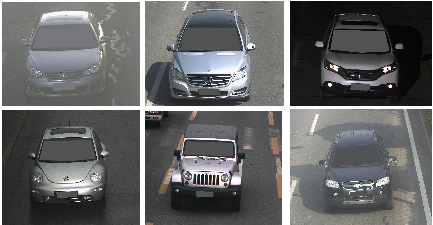
\includegraphics[width=0.5\linewidth]{figures/datasets/compcars_surveillance_samples.pdf}}
    \caption[\datasetname{CompCars} dataset]{Sample images of the surveillance-nature data from the \datasetname{CompCars} dataset. The images have considerable appearance variations due to the varying conditions of light, weather, traffic, etc. \externalsrc{\cite{Yang2015}}}
    \label{fig:DatasetCompCarsSurveillance}
\end{figure}

\begin{figure}[t]
    \centering
    \begin{subfigure}[b]{0.75\textwidth}
        \centering
        \includegraphics[width=\textwidth]{figures/datasets/compcars_speed.pdf}
        \caption[]{}
    \end{subfigure}
    \begin{subfigure}[b]{0.4\textwidth}
        \centering
        \includegraphics[width=\textwidth]{figures/datasets/compcars_side_front_views.pdf}
        \caption[]{}
    \end{subfigure}
    \hfill
    \begin{subfigure}[b]{0.4\textwidth}
        \centering
        \includegraphics[width=\textwidth]{figures/datasets/compcars_headlights.pdf}
        \caption[]{}
    \end{subfigure}
    \caption[Attributes of the \datasetname{CompCars} dataset]{Samples depicting various attributes of the \datasetname{CompCars} dataset. (a) shows the possibility to predict the maximum speed of a car, (b) shows different views of the same car, (c) shows the evolution of headlights of two different car models (years: $2006$ - $2014$). \externalsrc{\cite{Yang2015}}}
    \label{fig:DatasetCompCarsAttributes}
\end{figure}

% -------------------------------------------------------------------------------------------------
\subsection{PKU VehicleID}
\label{ssec:DatasetPKUVehicleID}

The \datasetname{VehicleID} dataset \cite{liu2016deep} (web: \cite{pkuvehicleiddataset}) contains data captured during daytime by multiple real-world surveillance cameras distributed in a small city. There are $26\ 267$ vehicles ($221\ 763$ images in total). Each image is attached with an ID label corresponding to its identity in the real world. In addition, there are manually labeled $10\ 319$ vehicles ($90\ 196$ images in total) of their vehicle model information (i.e. “MINI-cooper”, “Audi A6L”, “BWM 1 Series”, etc.). This dataset is usable thanks to the information about the model. We posit that at some point a hypothesis could be tested whether incorporating car model information into the machine learning model would improve its robustness. Nevertheless, only the front or rear view of the vehicle is available. This disadvantage is lessened by a reasonable number of training images. This dataset is also available only upon request and only for research purposes.

\begin{figure}[t]
    \centerline{\includegraphics[width=0.5\linewidth]{figures/datasets/vehicleid_overview.pdf}}
    \caption[\datasetname{VehicleID} dataset]{Few samples from the \datasetname{VehicleID} dataset. Each vehicle has at least two images in the dataset, but only its front and rear view were obtained. \externalsrc{\cite{liu2016deep}}}
    \label{fig:DatasetVehicleID}
\end{figure}

% -------------------------------------------------------------------------------------------------
\subsection{VeRI-776}
\label{ssec:DatasetVeRI776}

A large-scale benchmark dataset named \datasetname{VeRI-776} (web: \cite{veridataset}) for vehicle \gls{reid} in the real-world urban surveillance scenario \cite{Liu2018}. In our opinion, this dataset is one of the best available, and it already has been explored and served the purpose of training \gls{reid} models. However, one has to send an official request to retrieve a copy. The featured properties of this include the following important properties for training robust \gls{reid} models:

\begin{itemize}
    \item It contains over $50\ 000$ images of $776$ vehicles captured by $20$ cameras covering an $1\  \text{km}^2$ area in $24$ hours.
    
    \item The images were captured in a real-world unconstrained surveillance scene and labeled with varied attributes, e.g. \glspl{bbox}, types, colors, and brands.
    
    \item Each vehicle is captured by at least $2$ up to $18$ cameras in different viewpoints, illuminations, resolutions, and occlusions.
    
    \item Data samples are also labeled with license plates and other spatio-temporal information, such as the \glspl{bbox} of plates with corresponding strings, the timestamps of vehicles, and the distances between neighboring cameras.
\end{itemize}

\begin{figure}[t]
    \centerline{\includegraphics[width=\linewidth]{figures/datasets/veri776__overview.pdf}}
    \caption[\datasetname{VeRI-776} dataset]{The key properties of the \datasetname{VeRI-776} dataset. Individual vehicles offer rich within-class differences in different viewpoints. At the same time, different but similar vehicles may have trivial inter-class differences. Moreover, the license plates as the unique ID are at disposal for a vehicle search. Additional contextual information can assist in vehicle searches in the city. \externalsrc{\cite{Liu2018}}}
    \label{fig:DatasetVeRI776}
\end{figure}
